\chapter{Ladesysteme}
In diesem Kapitel werden die Ladesysteme für elektrische Busse erläutert. Im ersten Abschnitt werden Funktionsweise und EInsatzgeschichte der verschiednen Systeme erläutert. Im nächsten Abschnitt werden die betrachteten technischen Parameter definiert und in Abschnitt \ref{sec_tabellen_ladesysteme} ab Seite \pageref{sec_tabellen_ladesysteme} sind die ermittelten Parameter aufgelistet.

Ein \emph{Ladesystem} ist ein technisches System, das elektrische Energie aus dem öffentlichen Stromnetz in den Energiespeicher des Busses transportiert. Die \emph{Ladestrategie} beschreibt, wann, wo und wie lange geladen wird. Es kann über Nacht im Depot ("`Nachtladung"'), oder tagsüber an Haltestellen beziwhungsweise während der Fahrt geladen werden ("`Gelegenheitsladen"'). Rein technisch sind sehr viele Kombinationen von Ladesystem und Ladestrategie möglich, die betrieblich keinen Sinn machen – zum Beispiel der Einsatz eines aufwändigen Schnelladesystems für die Nachtladung im Depot. In dieser Arbeit werden Ladesysteme zusammen mit der für dieses System sinnvollen Ladestrategie betrachtet.

Die Ladesysteme werden nach drei Kriterien aufgeteilt:
\paragraph{Energietransport}
\begin{itemize}
	\item Konduktiv – es wird eine elektrisch Leitende Verbindung hergestellt
	\item Induktiv – die Energie wird durch schwingende Magnetfelder übertragen
	\item Batteriewechsel – die Batterie wird ausgewechselt
\end{itemize}

\paragraph{Fahrzustand}
\begin{itemize}
	\item Statisch – es wird nur geladen, während der Bus steht
	\item Dynamisch – die Batterie kann auch während der Fahrt aufgeladen werden
\end{itemize}

\paragraph{Automatisierungsgrad}
\begin{itemize}
	\item Manuell – Der Busfahrer seinen Arbeitsplatz verlassen, um den Ladevorgang zu beginnen und zu beenden\footnote{Denkbar ist auch, das der Fahrer im Bus bleibt und eine andere Person den Ladevorgang steuert. Solche Systeme existieren jedoch in Europa nicht.}
	\item Automatisch – Der Bus kann geladen werden, ohne das der Fahrer seinen Arbeitsplatz verlässt
\end{itemize}

\section{Untersuchte Systeme}
Für diese Arbeit wurden nur Ladesysteme betrachtet, bei denen bereits ein Testbetrieb im normalen Verkehr stattgefunden hat. In Tabelle \ref{uebersichtLadesysteme} sind die Namen der Systeme in normaler Schrift aufgeführt. Der Name des Herstellers ist \emph{kursiv} geschrieben. Sollte das System keinen eigenen Namen haben, wird der Name des Einsatzortes in \textsc{Kapitälchen} verwendet.
\marginpar{Irgendwas fehlt in \ref{uebersichtLadesysteme}. was?}
\begin{table}\centering
	\begin{tabularx}{\linewidth}{lp{2.1cm}p{2.1cm}XX}
		\toprule
		                           &                       \multicolumn{2}{c}{\textbf{Konduktiv}}                       & \textbf{Induktiv}                     & \textbf{Batteriewechsel}                \\
		\cmidrule{2-3}             & Manuell                                   & Automatisch                            & Automatisch                           & Automatisch                             \\ \midrule
		\multirow{12}{*}{Statisch} & IEC62196-2\newline\emph{BYD}              & Bůsbaar\newline\emph{Opbrid}           & IPT\newline\emph{Conductix"~Wampfler} & \textsc{Chattanooga}\newline\emph{AVS}  \\
		                           &                                           & FastFill\newline\emph{Proterra}        & primove\newline\emph{Bombardier}      & \textsc{Qingdao}\newline\emph{XJ Group} \\
		                           &                                           & \textsc{Hamburg}\newline\emph{Siemens} & WAVE\newline\emph{WAVE Inc.}          & \textsc{Shanghai}\newline\emph{Sunwin}  \\
		                           &                                           & TOSA\newline\emph{ABB}                 &                                       &  \\
		                           &                                           & \textsc{Shanghai}\newline\emph{Sunwin} &                                       &  \\
		                           &                                           & \textsc{Wien}\newline\emph{Siemens}    &                                       &  \\ \midrule
		\multirow{2}{*}{Dynamisch} & \textsc{Eberswalde}\newline\emph{Solaris} &                                        & OLEV\newline\emph{KAIST}              &  \\ \bottomrule
	\end{tabularx}
	\caption{Übersicht Ladesysteme}
	\label{uebersichtLadesysteme}
\end{table}

\subsection{Konduktive Ladesysteme} 
Bei konduktiven Systemen wird eine direkte Verbindung zwischen Stromführenden Metallteilen in Bus und Ladesystem hergestellt. Im Gegensatz zu Eisenbahnen, die über ihre Schienen permament geerdet sind müssen bei Bussen mindestens zwei Pole verbunden werden. Zum Schutz vor Fehlerströmen wird entweder eine doppelte Isolation mit Isolationsüberwachung oder ein weiterer Pol und FI-Schutzschalter verwendet.

\subsubsection{Manuell – Ladesteckdose}
Die in Elektroautos verwendeten Ladegeräte werden auch in Elektrobussen eingesetzt. Die Ladesysteme bestehen aus einer Ladesäule und einem Kabel mit einem Stecker, der in eine fahrzeugseitige Steckdose gesteckt wird. Die Stecker sind standardisiert und mit Kommunikationspfaden ausgestattet, über die Spannung und Strom ausgehandelt wird.

\textsc{BYD} verkauft Europa einen Elektrobus mit Ladestecker nach IEC 62196-2 ("`Mennekes"'). Durch die Verwendung von zwei Ladesteckern kann dieser Bus mit bis zu 80 kW geladen werden~\cite{bydSpecs4}.

Vorteil dieses Ladesystems ist die weite Kompatibilität. Ladestation und Bus können von unterschiedlichen Herstellern stammen. Die Ladestationen können sowohl von Bussen als auch von Elektroautos benutzt werden. Durch die relativ niedrige Ladeleistung und die fehlende Automatisierung ist dieses Ladesystem nur für das Aufladen über Nacht geeignet.

Viele Busse, die primär über andere Systeme geladen werden besitzen auch eine Ladesteckdose, um über Nacht oder abseits ihrer normalen Strecke geladen zu werden.\marginpar{Beleg!}

\subsubsection{Automatisiert – Stromabnehmer}
Um die elektrische Verbindung automatisch herzustellen werden ausfahrbare Stromabnehmer verwendet. Es gibt sowohl Systeme mit fahrzeugseitigem als auch mit stationsseitigem Stromabnehmer und jeweils unbeweglichen Kontakten auf der anderen Seite. In den meisten Ladesystemen liegen die zwei Pole auf demselben Stromabnehmer nebeneinander, \textsc{Opbrid} verwendet im \textsc{Bůsbaar}-System zwei Stromabnehmer vorne und hinten auf dem Bus und eine längs geteilte Stromschiene~\cite{SchKonLade}.

Mit diesen Systemen können hohe Leistungen übertragen werden, sie sind für die Aufladung des Busses an Endstationen (z. B. das System von Siemens in Wien~\cite{SiemensWien}) oder Zwischenhlatestellen (z. B. TOSA in Genf~\cite{tosa}) geeignet. 

Bei allen aktuellen Systemen befinden sich die Komponenten auf dem Dach des Busses, es müssen entweder Oberleitungen oder hohe Ladesäulen verwendet werden. Daher fallen diese Systeme im Stadtbild sehr auf. Einige Betreiber wünschen unauffälligere Systeme, für andere Betreiber sind die Ladesäulen jedoch als Symbol für die innovative Busse beliebt\marginpar{Beleg!}.

\subsubsection{Manuell/Automatisiert – Trolleybus}
In einigen Städten werden Trolleybusse mit Batterien ausgerüstet, um stromlose Abschnitte durchfahren zu können. Dies geschieht zum Beispiel in Rom und Lecce wo, in der denkmalgeschützten Altstadt keine Stromleitungen gebaut werden dürfen~\cite{tub_aleph001746639}[S. 66]. Auch eine Expansion des Liniennetzes in Vororten ohne Verlegung neuer Oberleitungen ist denkbar.

Dieses System ist eines von zwei \emph{dynamischen} Systemen, die die Aufladung während der Fahrt ermöglichen. Die Stromabnhemer können an speziellen Einfädelstellen automatisch ausgefahren werden, auf freier Strecke (z. B. nach einer Entgleisung der Stromabnehmer) muss der Fahrer sie jedoch mit Seilen oder Stangen an die Oberleitung führen. Da diese Systeme nur einen kleinen Teil ihrer Strecke ohne Oberleitung durchfahren, ist eine große Oberleitungsinfrastruktur erforderlich\marginpar{Belege!}. Kreuzungen zwischen Buslinien und besonders zwischen Bus- und Bahnlinien sind technisch sehr komplex.
                                 
\subsection{Induktive Ladesysteme}
An einer elektrischen Leiterschleife fällt eine Spannung an, wenn sich das Magnetfeld um die Leiterschleife verändert – entweder durch eine Änderung der Feldstärke oder Drehung der Schleife im Feld. Durch die Kombination von zwei Spulen kann so Wechselstrom von transportiert (und transformiert) werden. Im Transformator wird das Magnetfeld durch einen Eisenkern von der Primär- in die Sekundäsrpule geführt, nur ein kleiner Teil des Magnetfelds geht nicht durch die Sekundärspule.

Für die Ladung von Fahrzeugen kann kein Eisenkern verwendet werden und der Abstand zwischen den Spulen ist weit größer. Eine Sekundärspule wie im transformator wäre zu ineefiezient, von daher wird die Sekundärspule mit einem Kondensator zu einem Schwingkreis gekoppelt, dessen Resonanzfrequenz der Freqeunz der Primärspule entrichten~\cite{Kurs06072007}. Da die Frequenz der Primärspule weit über der Netzfrequenz von 50 oder 60 Hz liegt, ist ein Oszillator vor der Primärspule erforderlich. Über einen Gleichrichter hinter der Sekundärspule wird Gleichspannung bereitgestellt (siehe Abbildung \ref{abb_ResIndKopplung}).

\begin{figure}\centering
	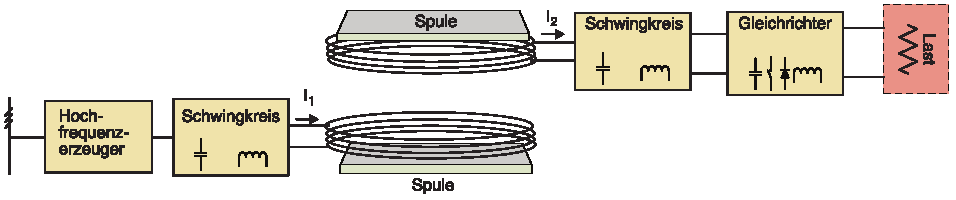
\includegraphics[width=\myFigureStandardWidth]{Resonant-Induktive_Kopplung}
	\caption{Blockdiagram eines induktiven Ladesystems. Nach: Chetvorno (Eigenes Werk) CC0, via Wikimedia Commons}
	\label{abb_ResIndKopplung}
\end{figure}

\subsubsection{Statisch}
Bei statischen Ladesystemen lädt der Bus im Stand an Haltestellen oder speziellen Ladestationen. Der Bus wird vom Fahrer anhand von Markierungen auf dem Boden ausgerichtet, teilweise wird die Sekundärspule näher an die Straße abgesenkt. Dadurch kann effizient geladen werden. Es gibt mehrere statische induktive Ladesysteme für Busse, die bereits seit Jahren im Einsatz sind~\cite{WeIPT}.

\subsubsection{Dynamisch}
Induktiv-dynamische Ladesysteme können die Batterie während der Fahrt aufladen, wenn sie über die ganze Strecke verlegt sind kann die Batterie sogar entfallen. Aufgrund der Bewegungen des Fahrzeuges während der Fahrt und aufgrund der Federung ist der durchschnittliche Abstand der Sekundärspule recht groß und damit die Effizienz niedrig~\cite{5618092}. Es werden nur die jeweils direkt unter dem Bus befindlichen Segmente der Primärspule eingeschaltet, was eine Aufteilung der Spule und Schalttechnologie unter der Straße erfordert.

\subsection{Batteriewechselsysteme}
Im Gegensatz zu den anderen Systemen wird bei Batteriewechselsystemen keine elektrische Energie in das Fahrzeug übertragen sondern die komplette Batterie ausgewechselt. Statt Energietransport findet hier also Stofftransport zwischen Ladestation und Bus statt. 

\section{Bewertungskriterien} \marginpar{Subsections}
\begin{itemize}
	\item Mechanik \marginpar{Bessere Beschreibung (Zeit ist nicht mechanisch)}
	\begin{description}
		\item \textbf{Abmaße, feste Position} \emph{Fahrzeug- uns Stationsseitig}\\
		Die Abmaße jener Komponenten des Ladesystems, deren Postion relativ zu ihrem Gegenüber fest ist.\\
		Beispiel: Pantograph und Stromschiene
		\item \textbf{Abmaße, freie Position} \emph{Fahrzeug- uns Stationsseitig}\\
		Die Abmaße jener Komponenten des Ladesystems, deren Postion frei gewählt werden kann.\\
		Beispiel: Elektrische Wandler
		\item \textbf{Masse} \emph{Fahrzeugseitig}\\
		Gesamtmasse der fahrzeugseitigen Komponenten
		\item \textbf{Freiheitsgrade} \emph{Fahrzeug- uns Stationsseitig}\\
		Anzahl der Freiheitsgrade, die eine bewegliche Komponente relativ zum Fahrzeug oder zur Station hat. 0, wenn es keine beweglichen Teile gibt.
		\item \textbf{Positionierungsgenauigkeit des Busses} \emph{Fahrzeugseitig} \\
		Erforderliche Genaugkeit der Positionierung des Busses relativ zur Ladestation, so dass noch 80\% der Standardladeleistung verfügbar ist. Besteht aus zwei translatorischen und zwei rotatorischen Komponenten (X, Y, Richtung des Busses, Kneelingwinkel)
		\item \textbf{Totzeit}\\
		Summe aus Zeit zwischen Halt des Busses und Ladebeginn sowie Zeit zwischen Ladeschluss und Abfahrt. Ist die Zeit von der Position abhängig, so wird jeweils eine Abweichung um die Hälfte des maximalen Wertes angenommen.
	\end{description}
	\item Elektrik
	\begin{description}
		\item \textbf{Anzahl der Wandler} \emph{Fahrzeug- und Stationsseitig}\\
		Anzahl der Komponenten, die den Spannungsverlauf verändern (Gleichrichter, Transformatoren etc.)
		\item \textbf{Spannung}\\
		Mit welcher Spannung wird geladen? Gleich- oder Wechselspannung? Nicht relevant bei induktiver Ladung und Batteriewechselsystemen.
		\item \textbf{Leistung}\\
		Aus dem öffentlichen Stromnetz erforderliche Leistung. Die im Bus angekommene Leistung ergibt sich durch die Effizienz. Es wird angenommen, das die Leistung aus dem ortsüblichen Niederspannungsnetz kommt. (400V Drehstrom in Europa)\marginpar{Amerika}
		\item \textbf{Effizienz}\\
		Prozentualer Anteil der Leistung, die im Fahrzeug am Laderegler ankommt.		
	\end{description}
	\item Sicherheit
	\begin{description}
		\item \textbf{Fehlerstromschutz}\\
		Wie wird vor Fehlerströmen geschützt?\\
		Beispiel: Fahrzeugseitige Isolationsüberwachung, RCD Typ B in Ladestation
		\item \textbf{Exponierte Leiter}\\
		Sind die spannungsführenden Leiter nur durch die umgebende Luft isoliert? Mögliche Antworten: nie, nur beim Ladevorgang, immer
		\item \textbf{Zugänglichkeit der Schnittstelle}\\
		Wo am Fahrzeug ist die Ladeschnittstelle? Wie ist sie geschützt?
		\item \textbf{Strahlung – Gesundheitsaspekte}\\
		\marginpar{Wie beschriebt man das? Macht es Sinn?}
		\item \textbf{Strahlung – EMV-Aspekte}\\
		\marginpar{Wie beschriebt man das? Macht es Sinn?}
		\item \textbf{Position der Ladestation}\\
		Ladesäule oder Unterflur? Im Depot oder an öffentlich zugänglicher Station?
	\end{description}
	\item Reife
	\begin{description}
		\item \textbf{Fahrzeugkilometer – Teststrecke}\\
		Mit diesem Ladesystem zurückgelegte Fahrzeugkilometer außerhalb des normalen Verkehrs. \marginpar{Formulierung}
		\item \textbf{Fahrzeugkilometer – Verkehr}\\
		Mit diesem Ladesystem im normalen Verkehr zurückgelegte Fahrzeugkilometer.
		\item \textbf{Erfahrungen der Vekehrsgesellschaften}\\
		War das System zuverlässig oder fehleranfällig? Hat sich die Zuverlässigkeit während des Betriebes verbessert?\marginpar{Macht es Sinn?}
	\end{description}
\end{itemize}

\section{Vergleichstabelle}
\label{sec_tabellen_ladesysteme}